\chapter{AVM Component Model}

\section{AVM Component by Example}
In order to better frame the description example AVM components from the ground vehicle domain are introduced. These will be used in the rest of this document to exemplify concepts described. 

\subsection{Engine}
An Engine (see figure \ref{Engine_Component}) serves as a good reference for an AVM component, as it spans cyber (electronic control) and physical, and encompasses multiple physics domains including mechanical, thermal, electrical, and acoustics. The Engine has physical interfaces through which it transfers energy (SAE-1/2 flywheel and flywheel housing), has mount points for installation, and has electronic interfaces for control. The Engine component has non-trivial dynamics and mode-based behavior that can be parameterized and modeled to predict the torque output, fuel consumption, and thermal output, as a function of mode, efficiency, engine-RPM, control settings, and a number of other parameters. The Engine has a complex geometry that can be captured with CAD models to analyze space claims, center-of-gravity, mass distribution, and mount point stresses using finite-element analyses. The Engine is also an example of a component which in itself is a highly complex system and made of several parts and sub-parts, but being a Commercial Off The Shelf (COTS) discrete component is treated as a black-box atomic component. The manufacturing model of such COTS components in AVM simply characterizes discrete attributes such as Cost, Lead Time, Shipping Volume, and Weight. 

% Do we need to say something about Caterpillar C-9 here OR we keep it general?? 
% need a second example
\begin{figure}
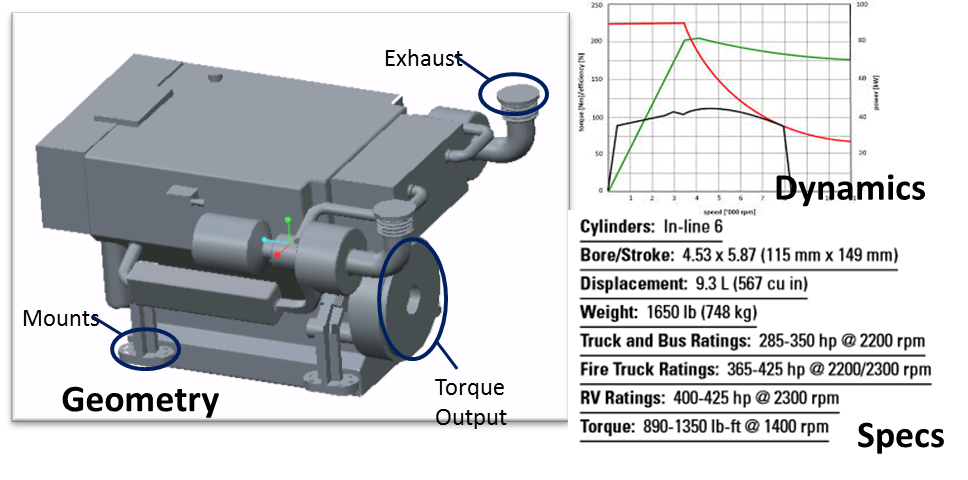
\includegraphics{Engine_Example}
\caption{Example Engine Component Models, Interfaces, and Specs}
\label{Engine_Component}
\end{figure}

\section{Component Model Organization}
The AVM Component Model being a multi-model is represented and persisted as a package containing all the artifacts (integration model, domain models, documentation, test articles) needed to use a component within the AVM tools. The integration model is the primary (and mandatory) artifact, and is often referred to as the AVM Component Model (with the acronym ACM) in the rest of this document.  

An AVM Component Package may include:
\begin{itemize}
\item AVM Component Model \emph{(required)}
\item Domain Models, such as:
\subitem CAD models
\subitem Modelica models
\subitem Manufacturing models
\item Supplemental artifacts such as:
\subitem Images
\subitem Diagrams
\subitem Documentation
\subitem Data Sheets
\end{itemize}

An AVM Component Package consists of a set of files that support a system designer's use of the AVM Component. These files may be arranged into a folder structure, but these folders must share a common root.

\begin{figure}
\fbox{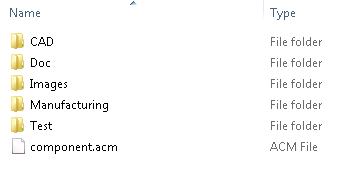
\includegraphics{ComponentPackage}}
\caption{Example Component Package contents}
\label{Component_Package}
\end{figure}

The ACM file serves dual purpose within the AVM Component package. It is the integration model that describes the component interface, references to domain models, and association with domain model ports, but it also serves as the package descriptor. Thus, an ACM file describing the component \textbf{must} be included within the root folder. It \textbf{must} have a file extension of ".acm" and be the only file with that extension in the root folder. No file other than the ACM is strictly required, but more files are typically included. All other files to be included in the component package \textbf{must} be referenced by "ResourceDependency" tags in the ACM file, with the exception of the ACM file itself.

Details of component distribution restrictions, licensing, and more must also be included in the ACM file. The ACM file is syntactically represented as an XML, and its schema is discussed in the following section.

